\documentclass[hidelinks,12pt]{article}
\usepackage[left=0.25cm,top=1cm,right=0.25cm,bottom=1cm]{geometry}
%\usepackage[landscape]{geometry}
\textwidth = 20cm
\hoffset = -1cm
\usepackage[utf8]{inputenc}
\usepackage[spanish,es-tabla]{babel}
\usepackage[autostyle,spanish=mexican]{csquotes}
\usepackage[tbtags]{amsmath}
\usepackage{nccmath}
\usepackage{amsthm}
\usepackage{amssymb}
\usepackage{mathrsfs}
\usepackage{graphicx}
\usepackage{subfig}
\usepackage{standalone}
\usepackage[outdir=./Imagenes/]{epstopdf}
\usepackage{siunitx}
\usepackage{physics}
\usepackage{color}
\usepackage{float}
\usepackage{hyperref}
\usepackage{multicol}
%\usepackage{milista}
\usepackage{anyfontsize}
\usepackage{anysize}
%\usepackage{enumerate}
\usepackage[shortlabels]{enumitem}
\usepackage{capt-of}
\usepackage{bm}
\usepackage{relsize}
\usepackage{placeins}
\usepackage{empheq}
\usepackage{cancel}
\usepackage{wrapfig}
\usepackage[flushleft]{threeparttable}
\usepackage{makecell}
\usepackage{fancyhdr}
\usepackage{tikz}
\usepackage{bigints}
\usepackage{scalerel}
\usepackage{pgfplots}
\usepackage{pdflscape}
\pgfplotsset{compat=1.16}
\spanishdecimal{.}
\renewcommand{\baselinestretch}{1.5} 
\renewcommand\labelenumii{\theenumi.{\arabic{enumii}})}
\newcommand{\ptilde}[1]{\ensuremath{{#1}^{\prime}}}
\newcommand{\stilde}[1]{\ensuremath{{#1}^{\prime \prime}}}
\newcommand{\ttilde}[1]{\ensuremath{{#1}^{\prime \prime \prime}}}
\newcommand{\ntilde}[2]{\ensuremath{{#1}^{(#2)}}}

\newtheorem{defi}{{\it Definición}}[section]
\newtheorem{teo}{{\it Teorema}}[section]
\newtheorem{ejemplo}{{\it Ejemplo}}[section]
\newtheorem{propiedad}{{\it Propiedad}}[section]
\newtheorem{lema}{{\it Lema}}[section]
\newtheorem{cor}{Corolario}
\newtheorem{ejer}{Ejercicio}[section]

\newlist{milista}{enumerate}{2}
\setlist[milista,1]{label=\arabic*)}
\setlist[milista,2]{label=\arabic{milistai}.\arabic*)}
\newlength{\depthofsumsign}
\setlength{\depthofsumsign}{\depthof{$\sum$}}
\newcommand{\nsum}[1][1.4]{% only for \displaystyle
    \mathop{%
        \raisebox
            {-#1\depthofsumsign+1\depthofsumsign}
            {\scalebox
                {#1}
                {$\displaystyle\sum$}%
            }
    }
}
\def\scaleint#1{\vcenter{\hbox{\scaleto[3ex]{\displaystyle\int}{#1}}}}
\def\bs{\mkern-12mu}



\title{La ecuación ordinaria de Legendre \\ {\large Tema 4}\vspace{-3ex}}
\author{M. en C. Gustavo Contreras Mayén}
\date{ }

\pagestyle{fancy}
\fancyhf{}
\rhead{Curso MAF}
\lhead{\leftmark}
\rfoot{\thepage}
\setlength{\headheight}{16pt}%

\def\changemargin#1#2{\list{}{\rightmargin#2\leftmargin#1}\item[]}
\let\endchangemargin=\endlist 


\begin{document}
\maketitle
\fontsize{14}{14}\selectfont
\tableofcontents
\newpage


\section{Avance en la solución.}

En el material de trabajo establecimos una EDO2H, tal que:
\begin{align}
\dv{x} \left[ (1 - x^{2}) \, \dv{F}{x} \right] + \left[ \lambda - \dfrac{m^{2}}{1 - x^{2}} \right] \, F(x) = 0
\label{eq:ecuacion_035}
\end{align}
Quedando dos casos: cuando $m = 0$ y $m \neq 0$.

\subsection*{Caso con \texorpdfstring{$m = 0$}{m=0}.}

Con $m = 0$, la ec. (\ref{eq:ecuacion_035}) se reduce a:
\begin{align}
(1 - x^{2}) \, \dv[2]{F}{x} - 2  \, x \, \dv{F}{x} + \lambda \, F(x) = 0
\label{eq:ecuacion_036}
\end{align}

\subsection*{Caso con \texorpdfstring{$m \neq 0$}{m  0}.}
Tendríamos entonces la siguiente EDO2H:
\begin{align}
\dv{x} \left[ (1 - x^{2}) \, \dv{F}{x} \right] + \left[ \lambda - \dfrac{m^{2}}{1 - x^{2}} \right] \, F(x) = 0
\label{eq:ecuacion_037}
\end{align}
Sin embargo, la forma más sencilla y elegante de obtener las soluciones es mediante el uso de operadores de escalera del momento angular.
\par
A continuación se revisará la solución para cada una de las ecuaciones diferenciales mencionadas, que veremos nos conducirán a los \emph{Polinomios ordinarios de Legendre} (con $m = 0$) y a los \emph{Polinomios Asociados de Legendre} (con $m \neq 0$).

\section{Funciones ordinarias de Legendre.}

La ecuación diferencial ordinaria de Legendre tiene la forma:
\begin{align}
(1 - x^{2}) \sderivada{y} - 2 \, x \, \pderivada{y} + \ell (\ell + 1) \, y = 0
\label{eq:ecuacion_18_01}
\end{align}
y tiene tres puntos singulares en $x = -1, 1, \infty$. Esta ecuación se presenta en diversos problemas de la física, en particular en problemas con simetría axial que involucra el operador $\nabla^{2}$, en donde se expresa en coordenadas esféricas.
\par
Normalmente la variable $x$ en la ecuación de Legendre es el coseno del ángulo en coordenadas polares, por lo que $-1 \leq x \leq 1$. El parámetro $\ell$ es un número real, y la solución a la ecuación (\ref{eq:ecuacion_18_01}) se le denomina \emph{función ordinaria de Legendre}.
\par
Es posible demostrar que $x = 0$ es un punto ordinario, por lo que podemos esperar dos soluciones linealmente independientes de la forma:
\begin{align*}
y = \sum_{n=0}^{\infty} a_{n} \, x^{n}
\end{align*}
Sustituimos entonces para encontrar:
\begin{align*}
\sum_{n=0}^{\infty} \left[ n \, (n - 1) a_{n} \, x^{n-2} - n \, (n - 1) \, a_{n} \, x^{n} - 2 \, n \, a_{n} \, x^{n} + \ell (\ell + 1) \, a_{n} \, x^{n} \right] = 0
\end{align*}
donde agrupamos los términos:
\begin{align*}
\sum_{n=0}^{\infty} \left[ (n + 2)(n + 1) \, a_{n+2} - [ n \, (n+1) - \ell (\ell + 1) ] \, a_{n} \right] \, x^{n} = 0
\end{align*}
La relación de recurrencia es por tanto:
\begin{align}
a_{n+2} = \dfrac{[n \, (n + 1)- \ell (\ell + 1)]}{(n + 1)(n + 2)} \, a_{n}
\label{eq:ecuacion_18_02}
\end{align}
para $n = 0, 1, 2, \ldots$
\par
Si elegimos $a_{0} = 1$ y $a_{1} = 0$ entonces obtenemos la solución:
\begin{align}
y_{1}(x) = 1 - \ell (\ell + 1) \dfrac{x^{2}}{2!} + (\ell - 2)\; \ell \; (\ell + 1)\;(\ell + 3) \dfrac{x^{4}}{4!} - \ldots
\label{eq:ecuacion_18_03}
\end{align}
Mientras que si escogemos $a_{0} = $ y $ a_{1} = 1 $, encontramos la segunda solución:
\begin{align}
y_{2}(x) = x - (\ell - 1)(\ell + 2) \dfrac{x^{3}}{3!} + (\ell - 3) (\ell - 1)(\ell + 2)(\ell + 4) \dfrac{x^{5}}{5!} - \ldots
\label{eq:ecuacion_18_04}
\end{align}

Aplicando la prueba de convergencia de la razón, se encuentra que ambas series convergen para $\abs{x} < 1$, y su radio de convergencia es unitario, que representa la distancia al punto singular más cercano de la ecuación. Dado que la ecuación (\ref{eq:ecuacion_18_03}) contiene sólo potencias pares de $x$ y la ecuación (\ref{eq:ecuacion_18_04}) contiene sólo potencias impares, esas dos soluciones no pueden ser proporcionales una de la otra, por lo tanto, son linealmente independientes. De aquí, la solución general para la ecuación (\ref{eq:ecuacion_18_01}) y con $\abs{x} < 1$ es:
\begin{align*}
y(x) = c_{1} \, y_{1} + c_{2} \, y_{2}
\end{align*}

\subsection{Funciones ordinarias de Legendre para enteros \texorpdfstring{$\ell$}{l}.}
En varios problemas de la física, el parámetro $\ell$ en la ecuación de Legendre - ec. (\ref{eq:ecuacion_18_01})- es un entero, es decir $\ell = 0,1,2,\ldots$. En ese caso, la relación de recurrencia - ec. (\ref{eq:ecuacion_18_02})- queda dada por:
\begin{align*}
a_{\ell + 2} = \dfrac{[ \ell (\ell + 1) - \ell (\ell + 1) ]}{(\ell + 1)(\ell + 2)} \, a_{\ell} = 0
\end{align*}
Esto es, la serie termina y obtenemos una solución con un polinomio de orden $\ell$. En particular, si $\ell$ es par, entonces $y_{1}(x)$ en la ecuación (\ref{eq:ecuacion_18_03}) se reduce a un polinomio, mientras que si $\ell$ es impar, lo mismo le ocurre a $y_{2}$ en la ecuación (\ref{eq:ecuacion_18_04}).
\par
Esas soluciones (adecuadamente normalizadas) son llamadas \emph{Polinomios ordinarios de Legendre de orden $\ell$}, se escriben $P_{\ell}(x)$ y son válidas para todo valor $x$ finito. De manera convencional, se normaliza $P_{\ell}(x)$ de tal manera que $P_{\ell}(1) =  1$, y como consecuencia $P_{\ell}(-1) = (-1)^{\ell}$. Los primeros polinomios se construyen fácilmente y están dados por:
\begin{center}
\begin{tabular}{l l}
$P_{0}(x) = 1 $ & $P_{1}(x) = 1 $ \\[0.5em]
$P_{2}(x) = \dfrac{1}{2} (3 x^{2} - 1)$ & $P_{3}(x) = \dfrac{1}{2} (5 x^{2} - 3 x)$ \\[0.5em] 
$P_{4}(x) = \dfrac{1}{8} (35 x^{4} - 30 x^{2} + 3)$ & $P_{5}(x) = \dfrac{1}{8} (63 x^{5} - 70 x^{3} + 15 x)$
\end{tabular}
\end{center}
\begin{figure}[H]
    \centering
    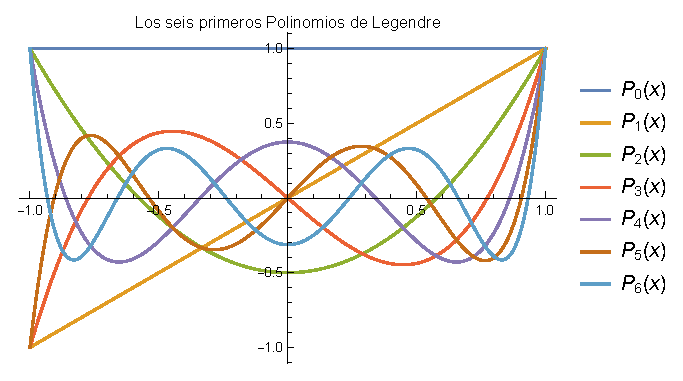
\includegraphics[scale=1.2]{Imagenes/Plot_Lagrange_0-6.eps}
    \caption{Gráfica de los primeros seis polinomios de Legendre.}
    \label{fig:polinomios_Lagrange_01}
\end{figure}
A pesar de que si $\ell$ es un entero par o impar, respectivamente para $y_{1}(x)$ - ec. (\ref{eq:ecuacion_18_03}) - o $y_{2}(x)$ - ec. (\ref{eq:ecuacion_18_04}), se termina dando un múltiplo del correspondiente polinomio ordinario de Legendre $P_{\ell}(x)$, la otra serie en cada caso no termina y por tanto converge sólo para $\abs{x} < 1$.
\par
Dependiendo de si $\ell$ es par o impar, se definen las \emph{funciones ordinarias de Legendre de segunda clase} como $Q_{\ell}(x) =  \alpha_{\ell} \, y_{2}(x)$ o $Q_{\ell}(x) =  \beta_{\ell} \, y_{1}(x)$, respectivamente, donde las constantes $\alpha_{\ell}$ y $\beta_{\ell}$ toman los valores:
\begin{align}
\alpha_{\ell} &= \dfrac{(-1)^{\ell/2} \; 2^{\ell} \; [(\ell / 2)!]^{2}}{\ell!} \hspace{3.5cm} \mbox{ para $\ell$ par} \label{eq:ecuacion_18_05}\\[1em]
\beta_{\ell} &= \dfrac{(-1)^{(\ell + 1)/2} \; 2^{\ell - 1} \; \lbrace \left[ (\ell - 1) /2 \right] ! \rbrace^{2}}{\ell!} \hspace{1cm} \mbox{ para $\ell$ impar} \label{eq:ecuacion_18_06}
\end{align}
La normalización de los factores se elige de tal manera que $Q_{\ell}(x)$ obedece la misma relación de recurrencia de $P_{\ell}(x)$.
\par
La solución general para la ecuación ordinaria de Legendre para enteros $\ell$ es por tanto:
\begin{align}
y(x) = c_{1} \, P_{\ell}(x) + c_{2} \, Q_{\ell} (x) 
\label{eq:ecuacion_18_07}
\end{align}
Donde $P_{\ell}(x)$ es un polinomio de orden $\ell$, que converge para cualquier $x$, y $Q_{\ell}(x)$ es una serie infinita que converge sólo si $\abs{x} < 1$.
\par
Usando el método del Wronkisano, podemos obtener una forma cerrada para $Q_{\ell}(x)$. Una segunda solución para la ecuación de Legendre -ec. \ref{eq:ecuacion_18_01}), con $\ell = 0$ es:
\begin{align}
\begin{aligned}[b]
y_{2}(x) &= P_{0}(x) \int^{x} \dfrac{1}{[P_{0}(u)]^{2}} \, \exp \left( \int^{u} \dfrac{2 \, v}{1 - v^{2}} \dd{v} \right) \dd{u} \\[0.5em]
&= \int^{x} \exp [ - \ln (1 - u^{2}) ] \dd{u} \\[0.5em]
&= \int^{x} \dfrac{\dd{u}}{(1 - u^{2})} = \dfrac{1}{2} \, \ln \left( \dfrac{1 + x}{1 - x} \right)
\end{aligned}
\label{eq:ecuacion_18_08}
\end{align}
En la segunda línea hemos utilizado el hecho de que $P_{0}(x)=1$.
\par
Lo que queda es ajustar la normalización de esta solución para que se corresponda con la ecuación (\ref{eq:ecuacion_18_05}). Expandiendo el logaritmo en la ec. (\ref{eq:ecuacion_18_08}) como una serie de Maclaurin, obtenemos
\begin{align*}
y_{2}(x) = x + \dfrac{x^{3}}{3} + \dfrac{x^{5}}{5} + \cdots \end{align*}
\begin{figure}[H]
    \centering
    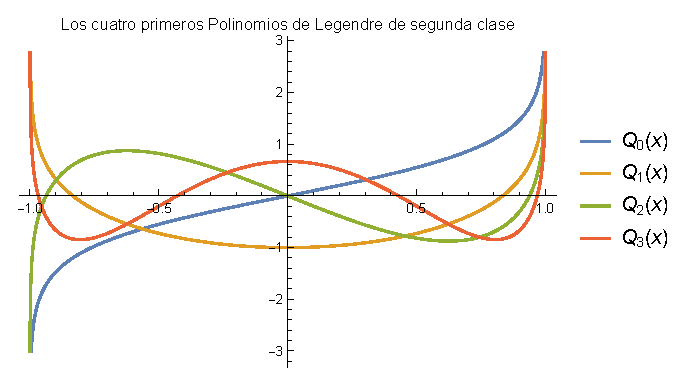
\includegraphics[scale=1.2]{Imagenes/Plot_LagrangeSC_0-4.eps}
    \caption{Gráfica de los cuatro polinomios de Legendre de segunda clase.}
    \label{fig:polinomios_Lagrange_02}
\end{figure}
Comparando esto con la expresión para $Q_{0}(x)$, usando la ec. (\ref{eq:ecuacion_18_04}) con $\ell = 0$ y normalizando -ec. (\ref{eq:ecuacion_18_05})-, encontramos que $y_{2}$ está correctamente normalizada, así:
\begin{align*}
Q_{0} (x) = \dfrac{1}{2} \, \ln \left( \dfrac{1 + x}{1 - x} \right)
\end{align*}
Usando el mismo método para $\ell = 1$, tenemos que:
\begin{align*}
Q_{1} (x) =  \frac{1}{2} \, x \,  \ln \left( \dfrac{1 + x}{1 - x} \right) - 1
\end{align*}
Se pueden encontrar formas cerradas para $Q_{\ell}(x)$ de mayor orden, usando la relacion de recurrencia.

\subsection{Propiedades de los Polinomios de Legendre.}

Como se mencionó anteriormente, cuando encontramos problemas físicos en donde la variable $x$ en la ecuación de Legendre es el coseno del ángulo polar $\theta$ en coordenadas esféricas, y entonces requiere la solución $y(x)$ que sea regular en $x = \pm 1$, que corresponde a $\theta = 0$ o $\theta = \pi$. Para que esto ocurra, requerimos que la ecuación tenga una solución polinomial, así el valor de $\ell$ debe ser un entero.
\par
Por otra parte, también requerimos que el coeficiente $c_{2}$ de la función $Q_{\ell}(x)$ en la ecuación (\ref{eq:ecuacion_18_07}) sea nulo, ya que $Q_{\ell}(x)$ es singular en $x = \pm 1$, como resultado de que la solución general es un múltiplo del polinomio de Legendre $P_{\ell}(x)$.

\subsection{Fórmula de Rodrigues.}

Como una ayuda para definir nuevas propiedades de los polinomios de Legendre, presentamos la \emph{fórmula de Rodrigues} para el $P_{\ell} (x)$:
\begin{align}
P_{\ell} (x) = \dfrac{1}{2^{\ell} \; \ell !} \dv[\ell]{x} \, (x^{2} - 1)^{\ell}
\label{eq:ecuacion_18_09}
\end{align}

\subsection{Ortogonalidad.}

Del Tema 3, reconocemos que la ecuación de Legendre es de la forma Sturm-Liouville con $p = 1 - x^{2}$, $q = 0$, $\lambda = \ell (\ell + 1)$ y $\omega = 1$, y que su intervalo natural es $[-1, 1]$. Ya que los polinomios ordinarios de Legendre $P_{\ell} (x)$ son regulares en los puntos extremos $x = \pm 1$, deben ser mutuamente ortogonales en este intervalo, es decir:
\begin{align}
\scaleint{6ex}_{\bs -1}^{1} P_{\ell}(x) \, P_{k}(x) \dd{x} = 0 \hspace{1cm} \mbox{ si $\ell \neq k$}
\label{eq:ecuacion_18_12}
\end{align}
Como ya se comentó previamente, la ortogonalidad mutua (y completitud) de $P_{\ell} (x)$ significa que cualquier función razonable $f(x)$ (es decir, una que satisfaga las condiciones de Dirichlet) puede expresarse en el intervalo de $\abs{x} < 1$ como una suma infinita de polinomios ordinarios de Legendre:
\begin{align}
f(x) = \nsum_{\ell = 0}^{\infty} a_{\ell} \, P_{\ell} (x)
\label{eq:ecuacion_013}
\end{align}
donde los coeficientes $a_{\ell}$ están dados por:
\begin{align}
a_{\ell} = \dfrac{2 \ell + 1}{2} \int_{-1}^{1} f(x) \, P_{\ell} (x) \dd{x}
\label{eq:ecuacion_18_14}
\end{align}

\subsection{Función generatriz.}

Una manera útil para manipular y estudiar secuencias de funciones o cantidades etiquetadas por una variable entera (en el caso de los polinomios de Legendre $P_{\ell} (x)$ están etiquetados por $\ell$), es mediante una función generatriz. 
\par
La función generatriz tiene quizás su mayor utilidad en el ámbito de la teoría de la probabilidad, sin embargo, también es de gran conveniencia en nuestro estudio.
\par
La función generatriz para decirlo, es una serie de funciones $f_{n} (x)$ para $n = 0, 1, 2,\ldots$ es una función $G (x, h)$ que contiene tanto a $x$, como una variable ficticia $h$, de tal manera que:
\begin{align*}
G(x,h) = \nsum_{n=0}^{\infty} f_{n} (x) \, h^{n}
\end{align*}
es decir, $f_{n}(x)$ es el coeficiente de $h^{n}$ en la expansión de $G$ en potencias de $h$. La utilidad de esta manera de trabajar la función, está en el hecho de que a veces es posible encontrar una forma cerrada para $G(x, h)$.
\par
En el caso de los polinomios ordinarios de Legendre, usemos las funciones $P_{n}(x)$ definidas por:
\begin{align}
G(x ,h) = (1 - 2 \, x \, h + h^{2})^{-1/2} =  \nsum_{n=0}^{\infty} P_{n}(x) \, h^{n}
\label{eq:ecuacion_18_15}
\end{align}
Como veremos las funciones así definidas son idénticas a los polinomios ordinarios de Legendre y la función $(1 - 2 \, x \, h + h^{2})^{-1/2}$ es de hecho la función generatriz para ellos. En el proceso también vamos a deducir varias relaciones útiles entre los diferentes polinomios y sus derivadas.
\par
Hacemos la anotación de que $\dv*{P_{n}(x)}{x}$ es $\ptilde{P}_{n}$, derivamos la ecuación (\ref{eq:ecuacion_18_15}) con respecto a $x$ y obtenemos:
\begin{align}
h (1 - 2 \, x \, h + h^{2})^{-3/2} = \sum \ptilde{P}_{n} \; h^{n}
\label{eq:ecuacion_18_16}
\end{align}
También derivamos la ecuación (\ref{eq:ecuacion_18_15}) con respecto a $h$ por lo que:
\begin{align}
(x - h) (1 - 2 \, x \, h + h^{2})^{-3/2} = \sum n \; P_{n} \; h^{n-1}
\label{eq:ecuacion_18_17}
\end{align}
La ecuación (\ref{eq:ecuacion_18_16}) puede re-escribirse usando la ecuación (\ref{eq:ecuacion_18_15}) como:
\begin{align*}
h \, \sum P_{n} \; h^{n} =  (1 - 2 \, x \, h + h^{2}) \sum \ptilde{P}_{n} \, h^{n}
\end{align*}
igualando los coeficientes de $h^{n+1}$, obtenemos la relación de recurrencia:
\begin{align}
P_{n} = \pderivada{P}_{n+1} - 2 \, x \; \pderivada{P}_{n} + \pderivada{P}_{n-1}
\label{eq:ecuacion_18_18}
\end{align}
Las ecuaciones (\ref{eq:ecuacion_18_16}) y (\ref{eq:ecuacion_18_17}) pueden combinarse como:
\begin{align*}
(x - h) \nsum \pderivada{P}_{n} \; h^{n} = h \, \nsum n \; P_{n} \; h^{n-1}
\end{align*}
donde el coeficiente de $h^{n}$ nos proporciona otra relación de recurrencia:
\begin{align}
x \, \pderivada{P}_{n} - \pderivada{P}_{n-1} =  n \; P_{n}
\label{eq:ecuacion_18_19}
\end{align}
eliminando $\pderivada{P}_{n-1}$ entre las ecuaciones (\ref{eq:ecuacion_18_18}) y (\ref{eq:ecuacion_18_19}), el resultado que se obtiene es:
\begin{align}
(n + 1) \, P_{n} = \pderivada{P}_{n+1} - x \; \pderivada{P}_{n}
\label{eq:ecuacion_18_20}
\end{align}
Si tomamos el resultado de la ecuación (\ref{eq:ecuacion_18_20}) reemplazando $n$ por $n-1$ y sumamos $x$ veces, obtenemos:
\begin{equation}
(1 - x^{2}) \, \pderivada{P}_{n} = n \; (P_{n-1} - x \, P_{n})
\label{eq:ecuacion_18_21}
\end{equation}
Finalmente, derivamos ambos lados con respecto a $x$ y usamos el resultado de la ecuación (\ref{eq:ecuacion_18_19}) para tener:
\begin{align*}
(1 - x^{2}) \sderivada{P}_{n} - 2 \, x \, \pderivada{P}_{n} &= n \, \bigg[ (\pderivada{P}_{n-1} - x \, \pderivada{P}_{n}) - P_{n} \bigg] = \\[0.5em]
&= n \, (-n \, P_{n} - P_{n}) = \\[0.5em]
&= -n \, (n + 1) \, P_{n}
\end{align*}
por lo que los $P_{n}$ definidos en la ecuación (\ref{eq:ecuacion_18_15}), satisfacen la ecuación ordinaria de Legendre.
\par
El ejemplo anterior muestra que las funciones $P_{n} (x)$ definida por la ecuación (\ref{eq:ecuacion_18_15}) satisfacen la ecuación ordinaria de Legendre con $\ell = n$ (un entero) y también de (\ref{eq:ecuacion_18_15}), estas funciones son regulares en $x = \pm 1$. Por lo tanto $P_{n}$ debe ser un múltiplo del n-ésimo polinomio ordinario de Legendre. Por lo tanto, sólo queda verificar la normalización. Esto se hace fácilmente en $x = 1$, cuando $G$ se convierte en:
\begin{align*}
G(1, h) = [(1 - h)^{2}]^{-1/2} =  1 + h + h^{2} + \cdots
\end{align*}
y podemos ver que todo $P_{n}$ así definido, se tiene $P_{n} (1) = 1$ como se requiere, por tanto son idénticos a los polinomios ordinarios de Legendre.
\par
Un uso particular de la función generatriz (\ref{eq:ecuacion_18_15}) es la representación del inverso de la distancia entre dos puntos en el espacio tridimensional en términos de polinomios ordinarios de Legendre. Si dos puntos $\vb{r}$ y $\ptilde{\vb{r}}$ se encuentran a distancias $r$ y $\ptilde{r}$, respectivamente, desde el origen, con $\ptilde{r} < r$, se tiene:
\begin{align}
\begin{aligned}[b]
\dfrac{1}{\abs{\vb{r} - \pderivada{\vb{r}}}} &= \dfrac{1}{(r^{2} + r^{\prime \: 2} - 2 \, r \, \pderivada{r} \, \cos \theta)^{1/2}} \\[0.5em]
&= \dfrac{1}{r \, [ 1 -2 (\pderivada{r}/r) \, \cos \theta + (\pderivada{r}/r)^{2}]^{1/2}} \\[0.5em]
&= \dfrac{1}{r} \nsum_{\ell = 0}^{\infty} \left( \dfrac{\pderivada{r}}{r} \right)^{\ell} \, P_{\ell} (\cos \theta)
\end{aligned}
\label{eq:ecuacion_18_22}
\end{align}
donde $\theta$ es el ángulo entre los dos vectores de posición $\vb{r}$ y $\ptilde{\vb{r}}$. Si $\ptilde{r} > r$, entonces $r$ y $\ptilde{r}$ deben de intercambiarse en la ecuación (\ref{eq:ecuacion_18_22}) o de lo contrario, la serie no converge.
\par
Este resultado puede ser utilizado por ejemplo, para escribir el potencial electrostático en un punto $\vb{r}$ debido a una carga $q$ en el punto $\ptilde{\vb{r}}$. Entonces, en el caso $\ptilde{r} < r$, se tiene que:
\begin{align*}
V(\vb{r}) = \dfrac{q}{4 \, \pi \, \varepsilon_{0} \, r} \nsum_{\ell=0}^{\infty} \left( \dfrac{\pderivada{r}}{r} \right)^{\ell} \, P_{\ell} (\cos \theta)
\end{align*}
Vemos el caso especial cuando la carga está en el origen, y $\pderivada{r} = 0$, entonces el término $\ell =0$ en la serie es no nulo, y la expresión se reduce a la forma ya conocida:
\begin{align*}
V(\vb{r}) = \dfrac{q}{4 \, \pi \, \varepsilon_{0} \, r}
\end{align*}

\subsection{Relaciones de recurrencia.}

En nuestro análisis previo de la función generatriz, derivamos varias relaciones de recurrencia útiles que satisfacen los polinomios ordinarios de Legendre $P_{n} (x)$. En particular, a partir de la ecuación (\ref{eq:ecuacion_18_18}), tenemos la cuarta relación de recurrencia:
\begin{align*}
\pderivada{P}_{n+1} + \pderivada{P}_{n-1} =  P_{n} + 2 \; x \; \pderivada{P}_{n}
\end{align*}
De las ecuaciones (\ref{eq:ecuacion_18_19}) a (\ref{eq:ecuacion_18_21}) tenemos las siguientes relaciones de recurrencia con tres términos:
\begin{align*}
\pderivada{P}_{n+1} &= (n+1) \; P_{n} + x \; \pderivada{P}_{n} \\[0.5em]
\pderivada{P}_{n-1} &= -n \; P_{n} + x \; \pderivada{P}_{n} \\[0.5em]
(1 - x^{2}) \, \pderivada{P}_{n+1} &= n \; (P_{n-1} - x \; P_{n}) \\[0.5em]
(2 \, n + 1) \, P_{n} &= \pderivada{P}_{n+1} - \pderivada{P}_{n-1}
\end{align*}

\subsection{Ejemplo.}

\textbf{Ejemplo 1.} Queremos encontrar la expansión de Legendre de una función $f(x)$ definida por:
\begin{align*}
f(x) = \begin{cases}
V_{0} & \mbox{ si } 0 < x \leq 1 \\[0.5em]
- V_{0} & \mbox{ si } -1 \leq x < 0
\end{cases}
\end{align*}
Utilizamos la ecuación (\ref{eq:ecuacion_18_14}) para determinar los coeficientes:
\begin{align*}
a_{\ell} &= \dfrac{2 \, \ell + 1}{2} \int_{-1}^{1} f(x) \, P_{\ell} (x) \dd{x} \\[0.5em]
&= \dfrac{2 \, \ell + 1}{2} \scaleint{6ex}_{\bs -1}^{0} \underbrace{f(x)}_{=-V_0}  P_{\ell} (x) \dd{x} + \dfrac{2 \, \ell + 1}{2} \scaleint{6ex}_{\bs 0}^{1} \underbrace{f(x)}_{=+V_0} \, P_{\ell} (x) \dd{x} \\[0.5em]
&= \dfrac{2 \, \ell + 1}{2} \, V_{0} \left[ - \scaleint{6ex}_{\bs -1}^{0} P_{\ell} (x) \dd{x} + \scaleint{6ex}_{\bs 0}^{1} P_{\ell} (x) \dd{x} \right]
\end{align*}
En la primera integral de la última línea, hacemos el cambio de variable $x = -y$, por lo que:
\begin{align*}
\scaleint{6ex}_{\bs -1}^{0} P_{\ell} (x) \dd{x} = \scaleint{6ex}_{\bs +1}^{0} P_{\ell} (-y) (-\dd{y}) = \scaleint{6ex}_{\bs 0}^{1} P_{\ell} (-y) \dd{y} = (-1)^{\ell} \, P_{\ell} (x) \dd{x}
\end{align*}
donde ocupamos una la propiedad de paridad de los polinomios ordinarios de Legendre:
\begin{align*}
P_{\ell} (-u) = (-1)^{\ell} \, P_{\ell} (u)
\end{align*}
Sustituimos en la expresión para los coeficientes:
\begin{align*}
a_{\ell} &= \dfrac{2 \, \ell + 1}{2} \, V_{0} \,  [1 - (-1)^{\ell} \scaleint{6ex}_{\bs 0}^{1} P_{\ell} (x) \dd{x} \\[0.5em]
&= \dfrac{2 \, \ell + 1}{2} \, V_{0} \begin{cases}
0 & \mbox{ si } \ell \mbox{ es par} \\[0.5em]
2 \, \displaystyle \scaleint{6ex}_{\bs 0}^{1} P_{2k+1} (x) \dd{x} & \mbox{ si } \ell = 2 k + 1 
\end{cases}
\end{align*}
donde para $\ell$ impar se definió como $\ell = 2 \, k + 1$ con $k = 0, 1, 2, \ldots$.
\par
Queda por evaluar la integral del polinomio de Legendre de orden impar en el intervalo $(0, 1)$. Para ello, utilizamos la fórmula de Rodrigues:
\begin{align*}
\scaleint{6ex}_{\bs 0}^{1} P_{2k+1} (x) \dd{x} &= \dfrac{1}{2^{2k+1} \; (2 \, k +1)!} \scaleint{6ex}_{\bs 0}^{1} \dv[2k+1]{x} \left[ (x^{2} {-} 1)^{2k+1} \right] \dd{x} = \\[0.5em]
&= \dfrac{1}{2^{2k+1} \; (2 \, k +1)!} \; \dv[2k]{x} \left[ (x^{2} {-} 1)^{2k+1} \right] \eval_{0}^{1} = \\[0.5em]
&= \dfrac{1}{2^{2k+1} \; (2 \, k +1)!} \; \bigg[ \dv[2k]{x} \left[ (x^{2} {-} 1)^{2k+1} \right] \eval_{x=1} + \\[0.5em]
&- \dv[2k]{x} \left[ (x^{2} {-} 1)^{2k+1} \right] \eval_{x=0} \bigg]
\end{align*}
El primer término resulta ser cero, porque no hay un número suficiente de diferenciaciones para deshacerse de todos los factores de $(x^{2} - 1)$. Para el segundo término, observamos que $(x^{2} - 1)^{2k + 1}$ es un polinomio en $x$ cuyos derivadas de varios órdenes, serán potencias de $x$. Estas potencias devolverán cero en $x = 0$, excepto para el término constante (de potencia cero). Por lo tanto, vamos a utilizar la expansión binomial para $(x^{2} - 1)^{2k + 1}$, que es igual a $-(1 {-} x^{2})^{2k + 1}$:
\begin{align*}
\dv[2k]{x} \left[ (x^{2} {-} 1)^{2k+1} \right] \eval_{x=0} &= - \dv[2k]{x} \left[ \sum_{j=0}^{2k+1} \dfrac{(2k+1)!}{j! \; (2k + 1 - j)!} \, (-x^{2})^{j} \right] \eval_{x=0} = \\[0.5em]
&= - \sum_{j=0}^{2k+1} \dfrac{(2k+1)!}{j! \; (2k + 1 - j)!} (-1)^{j} \, \dv[2k]{x} \left( x^{2j} \right) \eval_{x=0}
\end{align*}
de donde se obtiene un término constante cuando $k = j$, todos los demás términos de la suma se anulan ya sea por tener  demasiadas diferenciaciones (cuando $j < k$, terminamos derivando constantes), o por tener muy pocas diferenciaciones (cuando $j > k$, una potencia de $x$ permanece y se evalúa como cero en $x = 0$). Por tanto:
\begin{align*}
\dv[2k]{x} \left[ (x^{2} {-} 1)^{2k+1} \right] \eval_{x=0} &= - \dfrac{(2k+1)!}{k! \; (2k + 1)!} (-1)^{k} \, \dv[2k]{x} \left( x^{2k} \right) \eval_{x=0} \\[0.5em]
&= \dfrac{(2k+1)!}{k! \; (2k + 1)!} (-1)^{k+1} \; (2k)!
\end{align*}
Entonces el coeficiente $a_{2k+1}$ se escribe como:
\begin{align*}
a_{2k+1} = 2 \, \dfrac{2 \, (2 \, k + 1) + 1}{2} \; V_{0} \scaleint{6ex}_{\bs 0}^{1} P_{2k+1} (x) \dd{x} = \dfrac{(-1)^{k} \, (4 \, k + 3)(2 \, k!)}{2^{2k+1} \; k! \; (k+1)!} \, V_{0}
\end{align*}
con $a_{\ell} = 0$ para $\ell$ par. La expansión en series de la función $f(x)$ se escribe como:
\begin{align*}
f(x) = \begin{cases}
V_{0} & \mbox{ si } 0 < x \leq 1 \\[0.5em]
-V_{0} & \mbox{ si } -1 \leq x < 0
\end{cases}
= V_{0} \sum_{k=0}^{\infty} \dfrac{(-1)^{k}(4 \, k + 3)(2 \, k!)}{2^{2k+1} \; k! \; (k+1)!} P_{2k+1} (x)
\end{align*}
Expresando los primeros términos :
\begin{align*}
f(x) = V_{0} \left[ \dfrac{3}{2} \, P_{1}(x) - \dfrac{7}{8} \, P_{3}(x) + \dfrac{11}{16} \, P_{5}(x) - \cdots \right]
\end{align*}

\section{Ejercicios a cuenta.}


\noindent
%Ref. Arfken (2006) 12.1.3
\textbf{Ejercicio a cuenta (39). } Demuestra que el potencial electrostático producido por una carga $q$ en $z = a$ para $r < a$ es:
\begin{align*}
\varphi(\vb{r}) = \dfrac{q}{4 \pi \epsilon_{0} a} \, \nsum_{n=0}^{\infty} \left( \dfrac{r}{a} \right)^{n} \, P_{n}(\cos \theta)
\end{align*}
\\[0.5em]
\noindent

\textbf{Ejercicio a cuenta (40). } Una esfera conductora de calor de radio $a$ está compuesta por dos hemisferios con un espacio infinitesimal aislante entre ellos, como se muestra en la figura (\ref{fig:figura2}). Las mitades superior e inferior de la esfera están en contacto con baños térmicos de temperaturas $+ T_{1}$ y $-T_{1}$, respectivamente. La esfera de radio $a$ está dentro de otra esfera conductora de calor de radio $b$ con una temperatura $T_{2}$.
\begin{figure}[H]
    \centering
   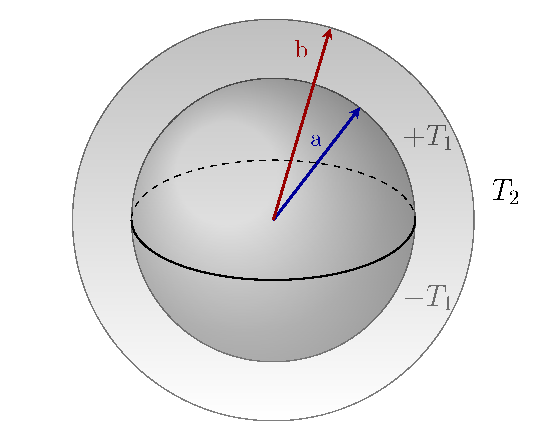
\includegraphics[scale=0.8]{Imagenes/esfera1.eps}
    \caption{Los hemisferios de la esfera interior se encuentran a diferentes temperatura.}
    \label{fig:figura2}
\end{figure}

Calcula la temperatura en los puntos:
\begin{enumerate}
\item Dentro de la esfera interior,
\item En la región entre las dos esferas, y
\item Por fuera de la esfera exterior.
\end{enumerate}

\noindent
%Arfken (2006) 12.3.3
\textbf{Ejercicio a cuenta (41). } Verifica la expansión de la función delta de Dirac:
\begin{align*}
\delta (1 - x) = \nsum_{n=0}^{\infty} \dfrac{2 \,n + 1}{2} \, P_{n} (x)
\end{align*}
\emph{Nota:} Considera que la función delta de Dirac queda cubierta completamente cuando se integra en el intervalo $[-1, 1]$.
\end{document}